\documentclass[aspectratio=169,11pt]{beamer}
% ==========================================================================
%  KSA lecture-slide theme  =  stock beamer "Boadilla"  +  KSA colour theme
%  brand colours sampled from the official KSA symbol mark:
%    Deep Prussian Blue  #2E3192   (지성 - intellect)
%    Golden Gray         #D6CBB1   (감성 - sensibility)
%  Engine: XeLaTeX.  Usage:
%    \documentclass[aspectratio=169,11pt]{beamer}
%    \input{../../theme/ksa-theme.tex}
%  Each deck lives in its own slides/kor/<deck>/ folder together with its
%  own images; ../../figs/ is kept only as a fallback for the shared cache.
% ==========================================================================

\usepackage{fontspec}
\usepackage{amsmath,amssymb}
\usepackage{graphicx}
\graphicspath{{figs/}{./}{../../../figs/}}
\usepackage{booktabs}
\usepackage{listings}
\usepackage{varwidth}

% ---- fonts (no ctex/xeCJK on this box -> fontspec drives CJK directly) -----
\defaultfontfeatures{Ligatures=TeX}
\setmainfont{Noto Sans CJK KR}
\setsansfont{Noto Sans CJK KR}
\setmonofont{Noto Sans Mono CJK KR}[Scale=0.92]

% ---- base theme: stock Boadilla ------------------------------------------
\usetheme{Boadilla}
\usefonttheme{professionalfonts}
\setbeamertemplate{navigation symbols}{}

% ---- KSA colour theme (recolour the stock theme) --------------------------
\definecolor{ksablue}{HTML}{2E3192}
\definecolor{ksabluedk}{HTML}{20226A}
\definecolor{ksagold}{HTML}{D6CBB1}
\definecolor{ksagolddk}{HTML}{A9976B}
\definecolor{ksared}{HTML}{C0392B}
\definecolor{ksagray}{HTML}{5B5B5B}

\setbeamercolor{structure}{fg=ksablue}
\setbeamercolor{alerted text}{fg=ksared}

\setbeamercolor{palette primary}{fg=white,           bg=ksablue}
\setbeamercolor{palette secondary}{fg=white,         bg=ksablue!85!black}
\setbeamercolor{palette tertiary}{fg=white,          bg=ksabluedk}
\setbeamercolor{titlelike}{fg=ksablue}
\setbeamercolor{frametitle}{fg=ksablue,bg=}
\setbeamercolor{title}{fg=ksablue}
\setbeamercolor{author}{fg=ksagray}
\setbeamercolor{institute}{fg=ksagray}
\setbeamercolor{block title}{fg=white,bg=ksablue}
\setbeamercolor{block body}{fg=black!85,bg=ksablue!6}
\setbeamercolor{item}{fg=ksablue}
\setbeamercolor{section in toc}{fg=black!85}

\setbeamerfont{frametitle}{series=\bfseries}
\setbeamerfont{title}{series=\bfseries}

% ---- footline:  KSA mark | "Made by ..." | n / N   (matches reference) ----
\newcommand{\ksacredit}{}
\setbeamertemplate{footline}{%
  \hbox{%
    \begin{beamercolorbox}[wd=.18\paperwidth,ht=2.6ex,dp=1.5ex,leftskip=1.1em]{}%
      \raisebox{-0.35ex}{\includegraphics[height=2.0ex]{ksa-logo.png}}%
    \end{beamercolorbox}%
    \begin{beamercolorbox}[wd=.64\paperwidth,ht=2.6ex,dp=1.5ex,center]{}%
      {\scriptsize\color{ksagray}\ksacredit}%
    \end{beamercolorbox}%
    \begin{beamercolorbox}[wd=.18\paperwidth,ht=2.6ex,dp=1.5ex,rightskip=1.1em]{}%
      \hfill{\scriptsize\color{ksablue}\insertframenumber\,/\,\inserttotalframenumber}%
    \end{beamercolorbox}%
  }%
  \vskip2pt
}

% ---- section divider: stock \sectionpage, KSA-coloured -------------------
\setbeamertemplate{section page}{%
  \begingroup\centering
    {\color{ksagolddk}\rule{0.16\paperwidth}{1pt}}\par\vskip1.0em
    {\usebeamerfont{title}\color{ksablue}\insertsectionhead\par}\vskip1.0em
    {\color{ksagolddk}\rule{0.16\paperwidth}{1pt}}\par
  \endgroup
}
\AtBeginSection[]{\begin{frame}[plain,noframenumbering]\vfill\sectionpage\vfill\end{frame}}

% ---- code listings ------------------------------------------------------------
\lstdefinestyle{ksa}{%
  basicstyle=\ttfamily\scriptsize,
  keywordstyle=\color{ksablue}\bfseries,
  commentstyle=\color{ksagray}\itshape,
  stringstyle=\color{ksagolddk},
  numberstyle=\tiny\color{ksagray},
  backgroundcolor=\color{ksablue!6},
  frame=leftline, framerule=1.4pt, rulecolor=\color{ksablue},
  xleftmargin=1em, aboveskip=0.8em, belowskip=0.4em,
  showstringspaces=false, breaklines=true, language=Python,
}
\lstset{style=ksa}

% ---- handy macros -----------------------------------------------------------
\newcommand{\kb}[1]{\textbf{\color{ksablue}#1}}   % blue keyword
\newcommand{\kq}[1]{\textbf{\color{ksared}#1}}    % red key-question

\setbeamerfont{title}{series=\bfseries,size=\fontsize{24}{30}\selectfont}
\setbeamerfont{subtitle}{series=\bfseries,size=\fontsize{14}{18}\selectfont}
\setbeamerfont{author}{size=\normalsize}
\setbeamerfont{institute}{size=\small}
\graphicspath{{figs/}{../../../../assets/}}
\makeatletter
\newcommand{\markpage}[1]{\protected@write\@auxout{}{\string\newlabel{#1}{{\the\c@framenumber}{}}}\hypertarget{#1}{}}
\newcommand{\pref}[1]{\hyperlink{#1}{\textcolor{ksagolddk}{(p.\ref{#1})}}}
\makeatother

\renewcommand{\ksacredit}{Machine Learning 1 \,\textperiodcentered\, 랜덤 포레스트}
\title{랜덤 포레스트 (Random Forest)}
\subtitle{서로 다른 나무 여럿의 다수결}
\author{Machine Learning 1}
\institute{한국과학영재학교 (KSA)}
\date{}
\begin{document}
\begin{frame}[plain,noframenumbering]\titlepage\end{frame}

% --- 오늘의 질문
\begin{frame}{오늘의 질문: 1906년 영국의 황소 무게 맞히기}
\vfill
\centering
{\Large 가축 품평회에서 \textbf{787명}이 황소 무게를 적어 냈다}\\[1.0em]
{\Large 답은 제각각. 그런데 가운데 값은 \kb{1,207 파운드}}\\[0.6em]
{\Large 실제 무게 (도축 후): \kq{1,198 파운드}}\\[1.0em]
{\large 한 명 한 명은 틀려도, 모으면 정답에 아주 가깝다 \qquad {\small (F. Galton, ``Vox Populi'', \textit{Nature}, 1907)}}
\vfill
\note{1906년 영국 플리머스의 가축 품평회에서 황소 무게 맞히기 대회가 열렸습니다. 787명이 답을 적어 냈고, 통계학자 프랜시스 골턴이 이 표를 모아 분석했습니다. 답은 제각각이었지만 가운데 값은 1207파운드, 실제 무게는 1198파운드로 1퍼센트도 차이 나지 않았습니다. 골턴은 이 결과를 1907년 네이처에 Vox Populi, 대중의 목소리라는 제목으로 발표했습니다. 한 명은 틀려도 여럿을 모으면 정답에 가까워진다. 오늘 배울 랜덤 포레스트는 이 아이디어를 결정 트리에 쓴 것입니다.}
\end{frame}

% --- 왜 모으면
\begin{frame}{모으면 왜 맞을까: 실수가 서로 달라야 한다}
\markpage{crowd}
\vfill
\centering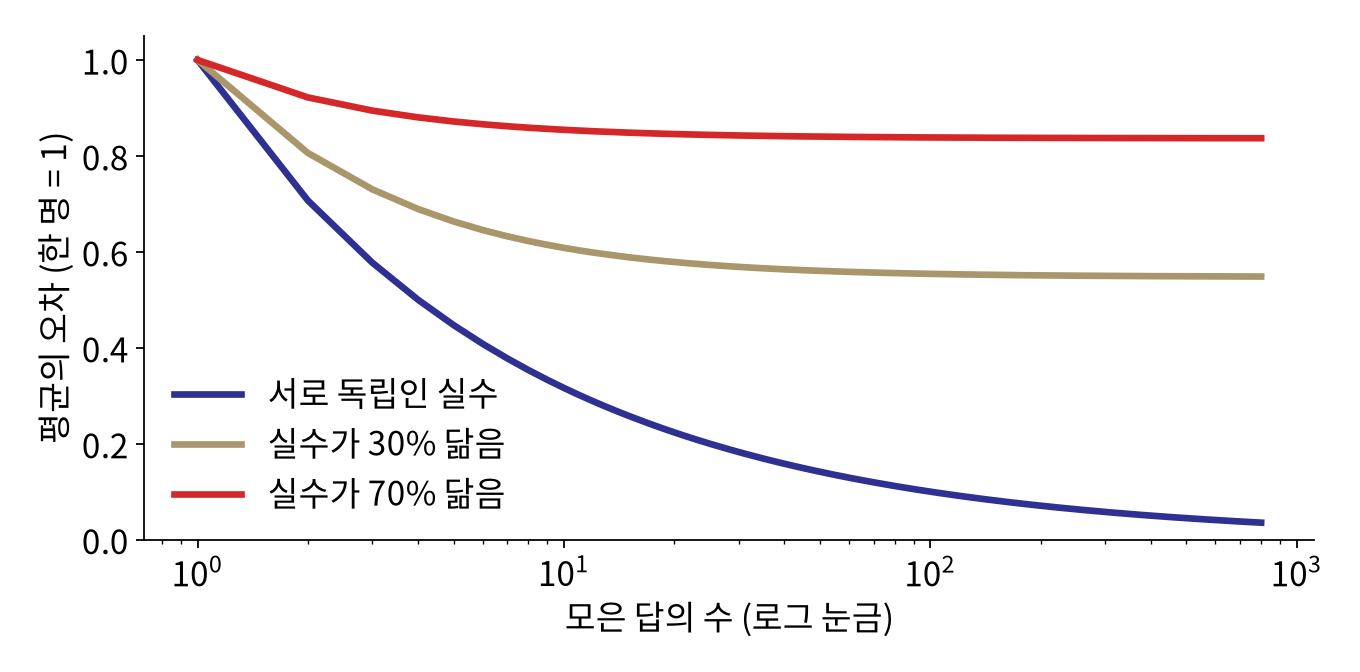
\includegraphics[width=0.52\linewidth]{rf_crowd.png}\par\vskip0.2em
{\Large\[ \text{평균의 오차} = \sigma\sqrt{\rho + \frac{1-\rho}{n}} \]}
{\large 독립 ($\rho = 0$) 이면 0 으로 \quad 같은 쪽으로 틀리면 ($\rho$ 큼) \kq{모아도 안 줄어든다}}
\vfill
\note{왜 모으면 맞을까요? 각자의 실수가 서로 다르면, 위로 틀린 사람과 아래로 틀린 사람이 상쇄되기 때문입니다. 식으로 쓰면, 한 명의 오차가 시그마이고 서로의 실수가 로 만큼 닮았을 때, n명의 답을 평균 낸 오차는 시그마 곱하기 루트 로 더하기 1 빼기 로 나누기 n입니다. 실수가 완전히 독립이면 n이 커질수록 0으로 갑니다. 그런데 실수가 닮을수록, 예를 들어 다들 같은 신문 기사를 읽고 같은 쪽으로 틀리면, 아무리 많이 모아도 로 만큼은 남습니다. 그래서 모을 때는 서로 다르게 틀리는 답을 모아야 합니다.}
\end{frame}

% --- 나무 한 그루
\begin{frame}{나무 한 그루는 불안정하다}
\vfill
\centering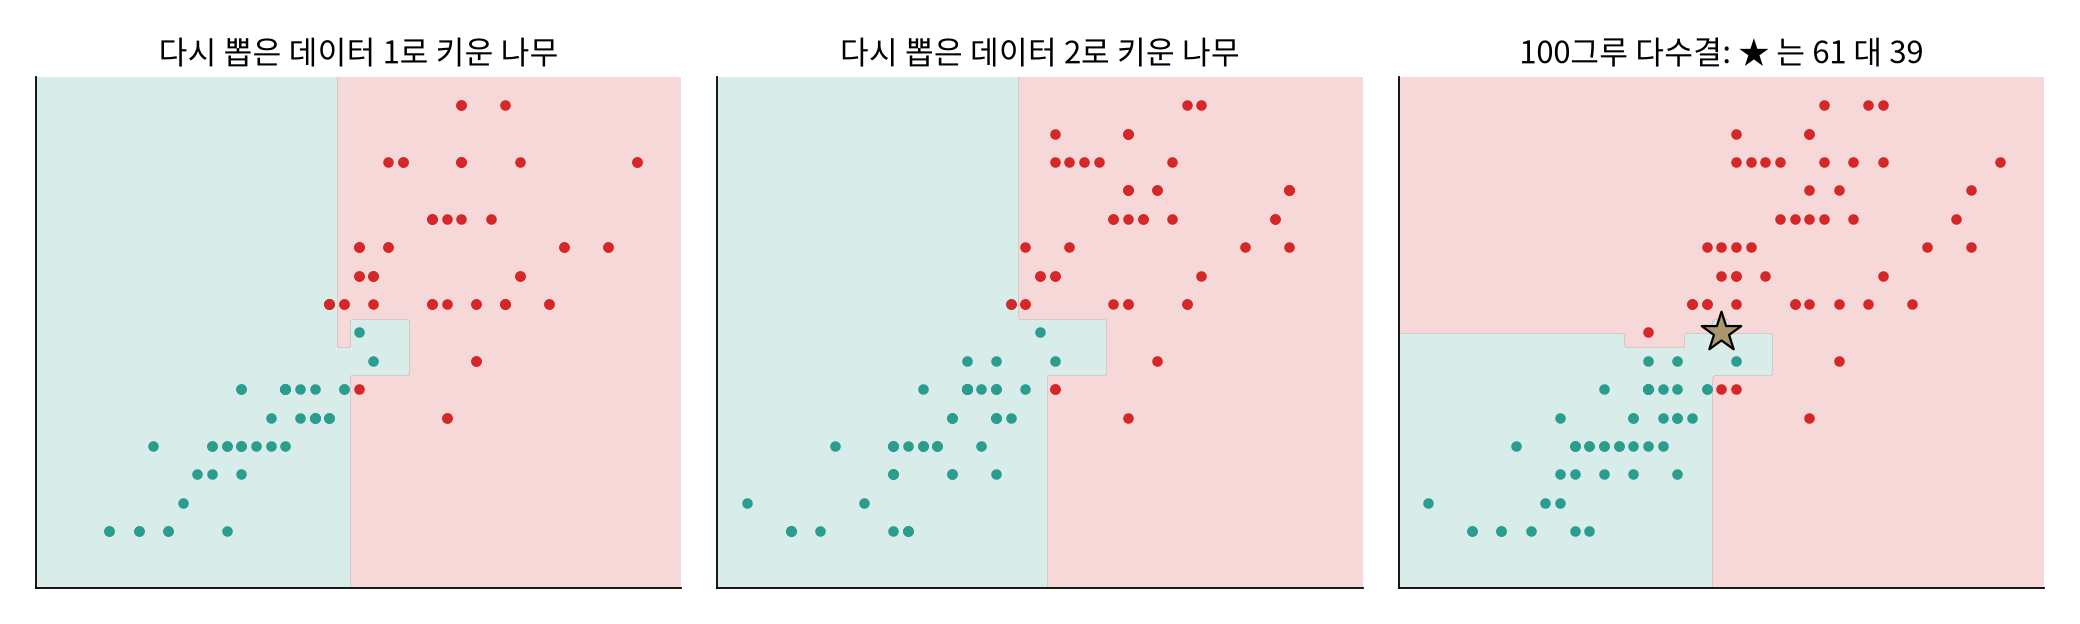
\includegraphics[width=0.96\linewidth]{rf_trees.png}\par\vskip0.2em
{\large 조금만 다르게 뽑아도 경계가 바뀐다 (왼쪽 둘) \quad 100그루를 모으면 \kb{부드러워진다}}
\vfill
\note{결정 트리 시간에 나무 한 그루는 불안정하다고 했습니다. 붓꽃 150송이에서 무작위로 다시 뽑은 데이터로 나무를 두 그루 키워 봤습니다. 왼쪽 두 그림을 보면 versicolor와 virginica 사이 경계가 서로 다릅니다. 우연히 뽑힌 몇 송이에 경계가 휘둘리는 겁니다. 하지만 바로 이 점이 쓸모 있습니다. 나무마다 실수가 다르니까요. 이렇게 조금씩 다른 나무를 100그루 키워 다수결을 내면 오른쪽처럼 경계가 부드러워집니다. 별 표시 꽃은 100그루 중 61그루가 versicolor, 39그루가 virginica라고 답했습니다.}
\end{frame}

% --- 부트스트랩
\begin{frame}{서로 다른 나무 만들기 1: 부트스트랩}
\markpage{boot}
\vfill
\centering
{\large 데이터 $m$ 개에서 \textbf{복원 추출}로 $m$ 개를 다시 뽑는다 (같은 것이 여러 번 뽑힐 수 있다)}\vskip0.6em
{\Large 카드 1 $\sim$ 10 에서 10번: \quad 9, 7, 6, 3, 4, 1, 1, 1, 2, 9}\\[0.4em]
{\large $\to$ 7 종류만 들어 있다 \quad 5, 8, 10 은 \kq{한 번도 안 뽑힘}}\vskip0.6em
{\Large\[ P(\text{한 번도 안 뽑힘}) = \Big(1 - \frac{1}{m}\Big)^m \approx \frac{1}{e} = 0.368 \]}
{\large 나무마다 데이터의 약 \kb{63\%} 로 학습 \quad 나머지 37\% 는 그 나무에게 처음 보는 데이터}
\vfill
\note{조금씩 다른 나무를 만드는 첫 번째 방법은 부트스트랩입니다. 데이터 m개에서 하나 뽑고 다시 넣고, 또 뽑고 다시 넣기를 m번 합니다. 카드 1부터 10까지로 해 보면 9, 7, 6, 3, 4, 1, 1, 1, 2, 9가 나왔습니다. 1은 세 번, 9는 두 번 뽑혔고, 5, 8, 10은 한 번도 안 뽑혔습니다. 데이터가 많으면 한 번도 안 뽑힐 확률이 1 빼기 m분의 1의 m제곱, 약 e분의 1, 37퍼센트가 됩니다. 그래서 나무마다 데이터의 약 63퍼센트로 학습하고, 나머지 37퍼센트는 그 나무에게는 처음 보는 데이터입니다. 이 사실을 잠시 뒤에 또 씁니다.}
\end{frame}

% --- 특징도 무작위
\begin{frame}{서로 다른 나무 만들기 2: 질문 후보도 무작위로}
\vfill
\centering
{\large 나무가 질문을 고를 때마다 특징 전부가 아니라 \textbf{무작위 일부}만 후보로 (분류는 보통 $\sqrt{d}$ 개)}\vskip0.8em
{\large 특징이 8개면 질문마다 \kb{$\sqrt{8} \approx 2$ 개}만 보고 고른다}\vskip0.8em
{\large 왜? 강한 특징 하나 (예: 혈당) 를 모든 나무가 첫 질문으로 써서 \kq{서로 닮는다}}\\[0.3em]
{\large $\to$ 가끔은 다른 특징으로 시작하게 해서 실수를 덜 닮게 만든다 \pref{crowd}}\vskip0.8em
{\small 부트스트랩 + 질문 후보 무작위 = 랜덤 포레스트 (L. Breiman, 2001; 앞서 T. K. Ho, 1995)}
\vfill
\note{두 번째 방법은 질문 후보도 무작위로 고르는 것입니다. 나무가 질문을 하나 고를 때마다 특징 전부를 보지 않고 무작위로 일부만 후보로 씁니다. 분류에서는 보통 특징 수의 제곱근만큼입니다. 특징이 8개면 2개 정도입니다. 왜 이렇게 할까요? 당뇨병 데이터의 혈당처럼 아주 강한 특징이 하나 있으면, 부트스트랩을 해도 모든 나무가 혈당을 첫 질문으로 써서 서로 닮게 됩니다. 앞에서 본 것처럼 실수가 닮으면 모아도 안 줄어듭니다. 그래서 가끔은 다른 특징으로 시작하게 해서 나무들을 덜 닮게 만듭니다. 이 두 가지를 합친 것이 2001년 레오 브라이먼이 정리한 랜덤 포레스트입니다.}
\end{frame}

% --- 다수결
\begin{frame}{예측: 다수결, 그리고 표의 비율}
\vfill
\centering
{\Large 꽃잎 길이 5.0, 너비 1.7 인 꽃 \quad $\to$ \quad versicolor \textbf{61} \; : \; virginica \textbf{39}}\\[1.0em]
{\large 답: versicolor \qquad 그리고 \kb{확신 61\%} 라는 것도 함께 알 수 있다}\\[0.6em]
{\large 92 : 8 이면 자신 있는 답, 51 : 49 면 사실상 모르는 답}\\[0.8em]
{\small 회귀 (숫자 예측) 는 다수결 대신 나무들의 예측을 \textbf{평균} \quad (골턴의 황소처럼)}
\vfill
\note{예측할 때는 나무마다 답을 내게 하고 다수결로 정합니다. 꽃잎 길이 5.0, 너비 1.7인 꽃은 versicolor 61표, virginica 39표라서 versicolor입니다. 표의 비율도 쓸모가 있습니다. 92 대 8이면 자신 있는 답이고, 51 대 49면 사실상 모른다는 뜻입니다. scikit-learn의 predict_proba가 이 비율을 줍니다. 숫자를 예측하는 회귀에서는 다수결 대신 나무들의 예측을 평균 냅니다. 골턴의 황소 무게처럼요.}
\end{frame}

% --- OOB
\begin{frame}{덤으로 얻는 검증: OOB (out-of-bag)}
\vfill
\centering
{\large 각 나무는 데이터의 약 37\% 를 \textbf{안 봤다} \pref{boot} \quad $\to$ 그 데이터로 채점할 수 있다}\vskip0.6em
{\large 데이터마다: 그 데이터를 안 본 나무들만 모아 다수결 $\to$ 맞았나?}\vskip0.8em
\renewcommand{\arraystretch}{1.3}
{\Large\begin{tabular}{lc}
당뇨병 768명, 나무 300그루 & 정확도\\\hline
OOB (따로 떼지 않음) & \kb{75.8\%}\\
5겹 교차 검증 & 75.7\%
\end{tabular}}\vskip0.6em
{\large 교차 검증을 따로 안 돌려도 거의 같은 추정 \quad scikit-learn \texttt{oob\_score=True}}
\vfill
\note{부트스트랩 덕분에 덤이 하나 있습니다. 각 나무는 데이터의 약 37퍼센트를 학습에 쓰지 않았습니다. 그러니 데이터 하나하나에 대해, 그 데이터를 안 본 나무들만 모아 다수결을 내서 맞았는지 채점할 수 있습니다. 이를 out-of-bag, OOB 점수라고 합니다. 당뇨병 환자 768명에 나무 300그루로 해 보면 OOB 정확도 75.8퍼센트, 5겹 교차 검증 75.7퍼센트로 거의 같습니다. 교차 검증을 따로 돌리지 않아도 성능을 추정할 수 있는 겁니다.}
\end{frame}

% --- 나무 수
\begin{frame}{나무를 늘리면}
\markpage{ntrees}
\vfill
\centering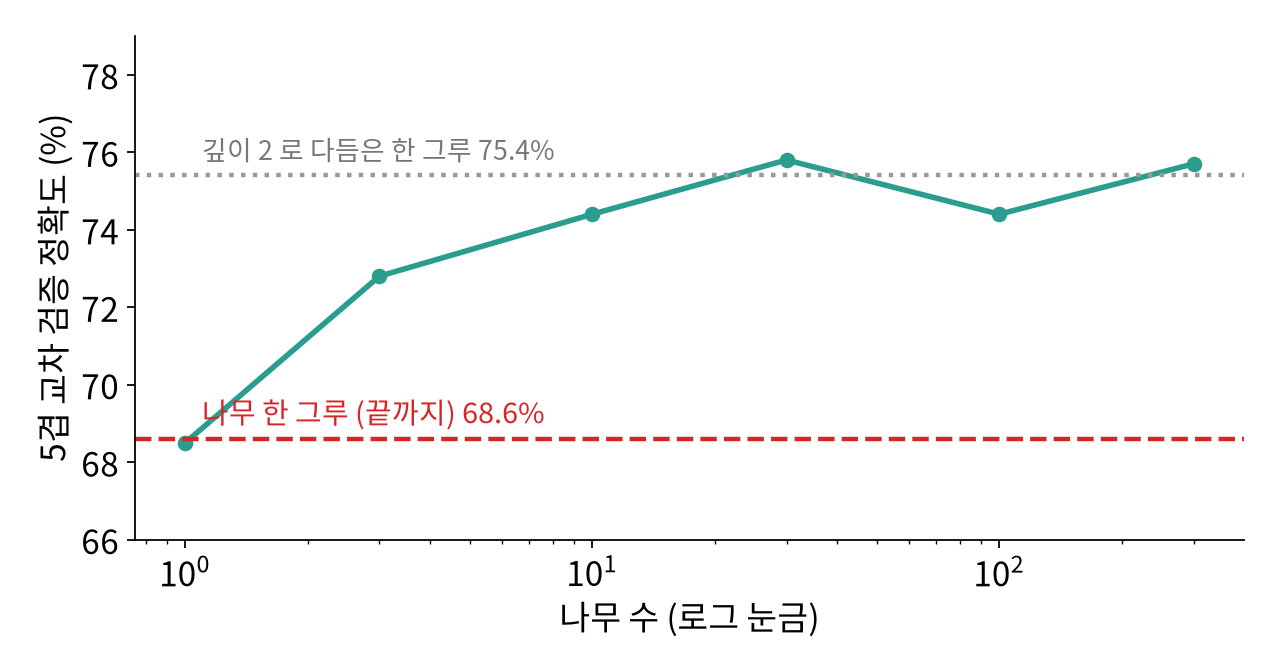
\includegraphics[width=0.58\linewidth]{rf_ntrees.png}\par\vskip0.2em
{\large 한 그루 \kq{68.6\%} $\to$ 숲 300그루 \kb{75.7\%} \quad (다듬은 한 그루 75.4\% 만큼, \textbf{튜닝 없이})}\\[0.2em]
{\small 나무를 늘려도 과대적합되지 않는다 (평균이 안정될 뿐) \quad 대신 계산 시간이 는다}
\vfill
\note{당뇨병 데이터에서 나무 수를 늘려 봤습니다. 끝까지 키운 나무 한 그루는 교차 검증 68.6퍼센트였습니다. 숲은 나무 수가 늘수록 올라 30그루 근처부터 75퍼센트대에서 안정됩니다. 결정 트리 시간에 깊이를 교차 검증으로 골라 다듬은 한 그루가 75.4퍼센트였는데, 숲은 깊이 같은 걸 고르지 않고도 그만큼 나옵니다. 그리고 나무를 늘려도 과대적합되지 않습니다. 평균이 더 안정될 뿐입니다. 나무가 많을수록 손해 보는 건 계산 시간뿐이라 보통 100에서 500그루를 씁니다.}
\end{frame}

% --- 특징 중요도
\begin{frame}{어떤 특징이 중요했나}
\vfill
\centering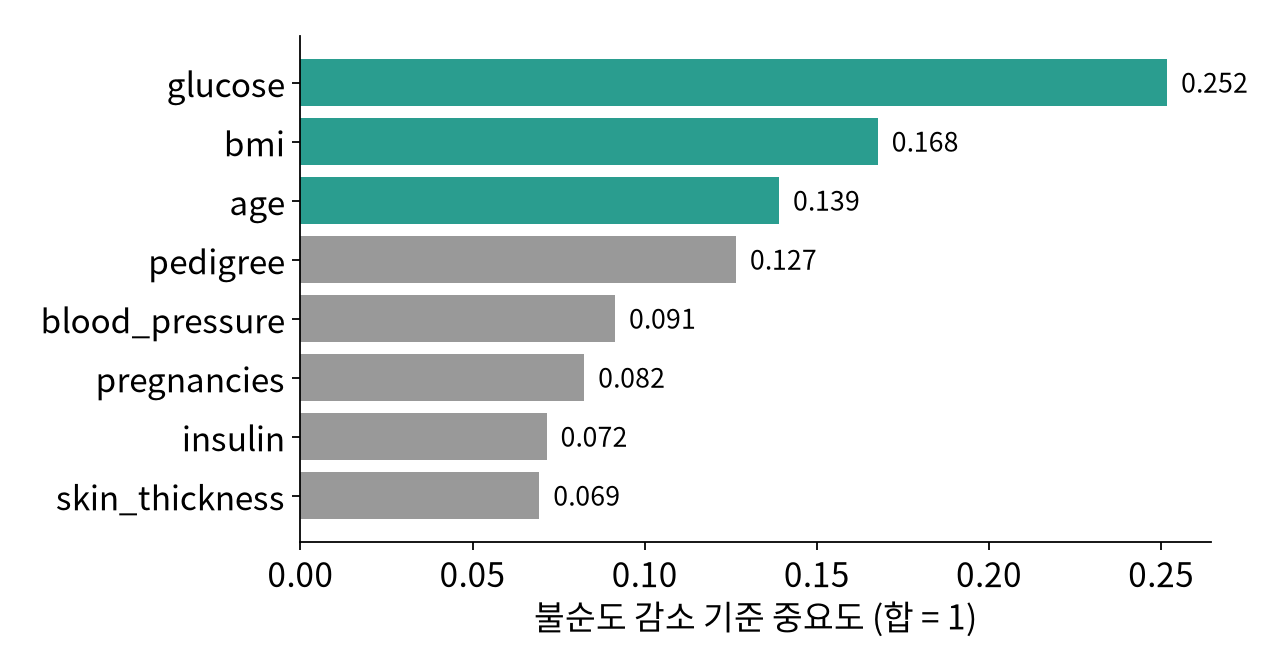
\includegraphics[width=0.56\linewidth]{rf_importance.png}\par\vskip0.2em
{\large 특징마다 \textbf{불순도를 줄인 양}을 모든 나무에서 더한다 \quad 혈당 · BMI · 나이 순}\\[0.2em]
{\small 주의: 값의 종류가 많은 특징을 과대평가하는 경향 $\to$ 다음 시간 SHAP 로 더 정확히}
\vfill
\note{랜덤 포레스트는 나무가 수백 그루라 결정 트리처럼 한눈에 읽을 수는 없습니다. 대신 특징 중요도를 줍니다. 각 특징이 질문으로 쓰일 때마다 불순도를 얼마나 줄였는지 모든 나무에서 더한 값입니다. 당뇨병에서는 혈당이 0.252로 가장 중요하고, BMI, 나이 순입니다. 의학적으로도 그럴듯합니다. 다만 이 방법은 값의 종류가 많은 특징을 실제보다 중요하게 보는 경향이 있어서, 다음 시간에 배울 SHAP으로 더 정확하게 봅니다.}
\end{frame}

% --- 장단점
\begin{frame}{랜덤 포레스트의 장점과 약점}
\vfill
\centering
\renewcommand{\arraystretch}{1.5}
{\large\begin{tabular}{ll}
\kb{장점} & 튜닝을 거의 안 해도 잘 된다 \quad 과대적합에 강하다 \quad OOB · 특징 중요도 덤\\
 & 표준화 불필요, 나무끼리 독립이라 \textbf{병렬}로 빠르게 키울 수 있다\\
\kq{약점} & 한 그루처럼 읽을 수는 없다 \quad 모델이 크다 (나무 수백 그루)\\
 & 학습 범위 밖의 값은 예측 못 한다 (나무는 본 값의 평균만 낸다)
\end{tabular}}\vskip0.8em
{\large 표 데이터에서는 지금도 가장 먼저 시도해 볼 만한 모델 \quad 다음: 나무를 \textbf{차례로} 쌓는 GBDT}
\vfill
\note{정리하면, 랜덤 포레스트는 튜닝을 거의 안 해도 잘 되고, 과대적합에 강하고, OOB 점수와 특징 중요도를 덤으로 줍니다. 표준화도 필요 없고, 나무끼리 독립이라 여러 CPU로 동시에 키울 수 있습니다. 약점은 한 그루처럼 규칙을 읽을 수 없고, 모델이 크고, 학습 데이터 범위 밖의 값은 예측하지 못한다는 겁니다. 그래도 표 형태의 데이터라면 지금도 가장 먼저 시도해 볼 만한 모델입니다. 다음 시간에는 나무를 동시에가 아니라 차례로 쌓아서 앞 나무의 실수를 고쳐 가는 GBDT를 배웁니다.}
\end{frame}

% --- 문제풀이
\begin{frame}{문제풀이}
\vfill
\begin{enumerate}
\item 데이터 4개 \{A, B, C, D\} 에서 부트스트랩으로 4개를 뽑았더니 B, B, D, A 였다. 이 나무의 OOB 데이터는?\vskip0.8em
\item 나무 5그루가 각각 ``고양이, 개, 고양이, 고양이, 개'' 라고 답했다. 숲의 답과 확신은?\vskip0.8em
\item 한 명의 오차가 10 kg, 실수의 상관이 0 일 때 100명의 평균 오차는? 상관이 0.5 면?\vskip0.8em
\item 특징이 100개인 분류 문제에서 랜덤 포레스트는 질문마다 보통 몇 개의 특징을 후보로 보나?
\end{enumerate}
\vfill
\note{1번 답. 한 번도 안 뽑힌 C입니다. 2번 답. 고양이 3표, 개 2표라서 고양이, 확신 60퍼센트입니다. 3번 답. 상관이 0이면 10 곱하기 루트 100분의 1, 1kg입니다. 0.5면 10 곱하기 루트 0.5 더하기 0.005, 약 7.1kg으로 거의 안 줄어듭니다. 4번 답. 제곱근, 10개입니다.}
\end{frame}

% --- 실습
\begin{frame}{실습}
\vfill
\centering\begin{tabular}{rl}
\large 1 & 부트스트랩 + 나무 + 다수결로 숲 직접 만들기 $\to$ 61 : 39 같은 표 세어 보기\\[0.5em]
\large 2 & OOB 점수 직접 계산 vs \texttt{oob\_score\_}, 나무 수에 따른 정확도\\[0.5em]
\large 3 & 실제 데이터: 당뇨병 · 타이타닉에서 한 그루 vs 숲, 특징 중요도
\end{tabular}\vskip1em
Pima Indians Diabetes (UCI) · Titanic (seaborn-data) \\[0.4em]\href{https://colab.research.google.com/github/SuminHan/book-ml/blob/main/slides/v2/ml1/week07/random_forest/lab/random_forest.ipynb}{\textcolor{ksagolddk}{▶ Colab에서 실습 노트북 열기}}
\vfill
\note{실습은 세 부분입니다. 첫째, 부트스트랩으로 데이터를 다시 뽑고 결정 트리를 여러 그루 키워 다수결을 내는 숲을 직접 만들어 봅니다. 둘째, OOB 점수를 직접 계산해서 scikit-learn의 oob_score와 비교하고, 나무 수에 따라 정확도가 어떻게 변하는지 그립니다. 셋째, 당뇨병과 타이타닉 데이터에서 한 그루와 숲을 비교하고 특징 중요도를 읽어 봅니다.}
\end{frame}

% --- 정리
\begin{frame}{정리}
\vfill
\centering\large\begin{tabular}{l}
여럿의 답을 모으면 정확해진다 \quad 단, \textbf{실수가 서로 달라야} 한다 (골턴 1907)\\[0.5em]
\textbf{랜덤 포레스트} = 부트스트랩 + 질문 후보 무작위 ($\sqrt d$) 로 서로 다른 나무 + 다수결\\[0.5em]
표의 비율 = 확신 \quad 안 본 37\% 로 \kb{OOB} 검증\\[0.5em]
한 그루 68.6\% $\to$ 숲 75.7\% (당뇨병) \quad 나무를 늘려도 과대적합 없음
\end{tabular}
\vfill
\note{정리합니다. 여럿의 답을 모으면 정확해지지만, 실수가 서로 달라야 합니다. 골턴의 황소가 보여 준 것입니다. 랜덤 포레스트는 부트스트랩과 질문 후보 무작위로 서로 다른 나무를 여럿 키워 다수결을 냅니다. 표의 비율은 확신을 알려 주고, 각 나무가 안 본 37퍼센트로 OOB 검증을 덤으로 얻습니다. 당뇨병 데이터에서 한 그루 68.6퍼센트가 숲으로 75.7퍼센트가 됐고, 나무를 늘려도 과대적합되지 않습니다.}
\end{frame}
\end{document}
